\documentclass[11pt]{article}
\usepackage[top=1in, bottom=0.5in, left=1in, right=1in]{geometry}
\usepackage[T1]{fontenc}
\usepackage[polish]{babel}
\usepackage[utf8]{inputenc}
\usepackage{lmodern}
\selectlanguage{polish}
\usepackage{graphicx}
\begin{document}
\title{Laboratorium 3}
\author{Jan Seredyński}
\date{\today}
\maketitle

\section{Wstęp}
Zadaniem laboratorium jest pomiar czasu wykonania operacji wypelnienia stosu. Do wykonania analizy zstosowałem trzy implementacje:dwie tablicowe i jedna oparta na liście.


\section{Schematy odpowiednich struktur}

Lista dwukierunkowa
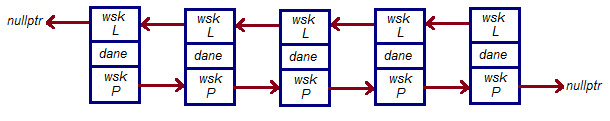
\includegraphics[width=5in]{lista2_1.png} 
\par\vspace{\baselineskip}
\hrule
\par\vspace{\baselineskip}
Stos, kolejka
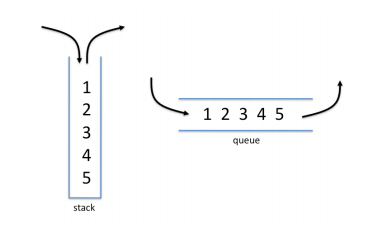
\includegraphics[width=3in]{stackqueue.png} 
\newpage

\section{Wydajność stosu na tablicy}
Podczas tej próby stos jest opraty na tablicy dynamicznej, która przy każdym pushowaniu twory nową tablice większą o 1, a następnie kopiuje pozostałe elementy do nowoutworznej tablicy, a na końcu wpisuje nowy element.\\\
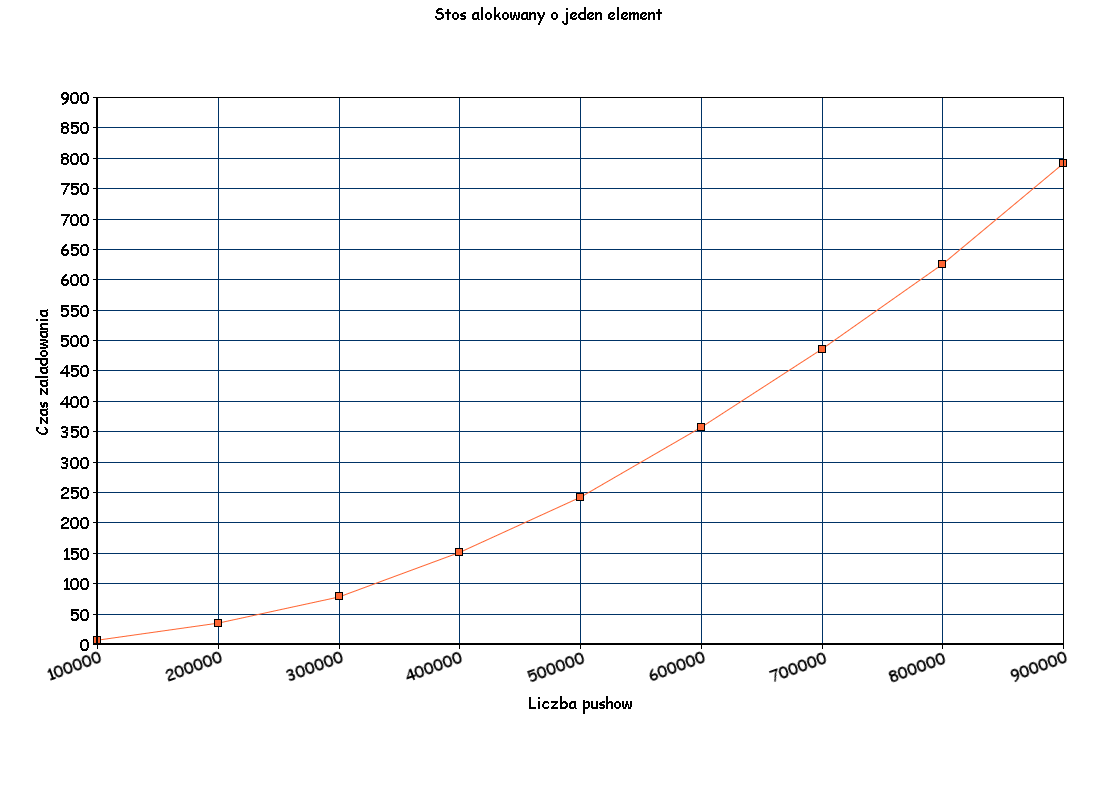
\includegraphics[width=6.5in]{3stos_dyn_o_1.png}
Na podstawie wykresu można stwierdzić, że ta implementacja ma przyrost geometryczny - kwadratowy.
\section{Wydajność stosu na tablicy i liscie}
Podczas tej próby stos jest opraty na tablicy dynamicznej, która przy każdym pushowaniu sprawdza czy tablica pomieśći nowy element, a gdy jest potrzeba zaalokowania nowej pamięci tworzy nową tablice większą o 100\%, a następnie kopiuje pozostałe elementy do nowoutworznej tablicy, a na końcu pushuje nowy element.\\\
Na tym samym wykresie została również złożoność obliczeniowa przy implementacji listy.\\\
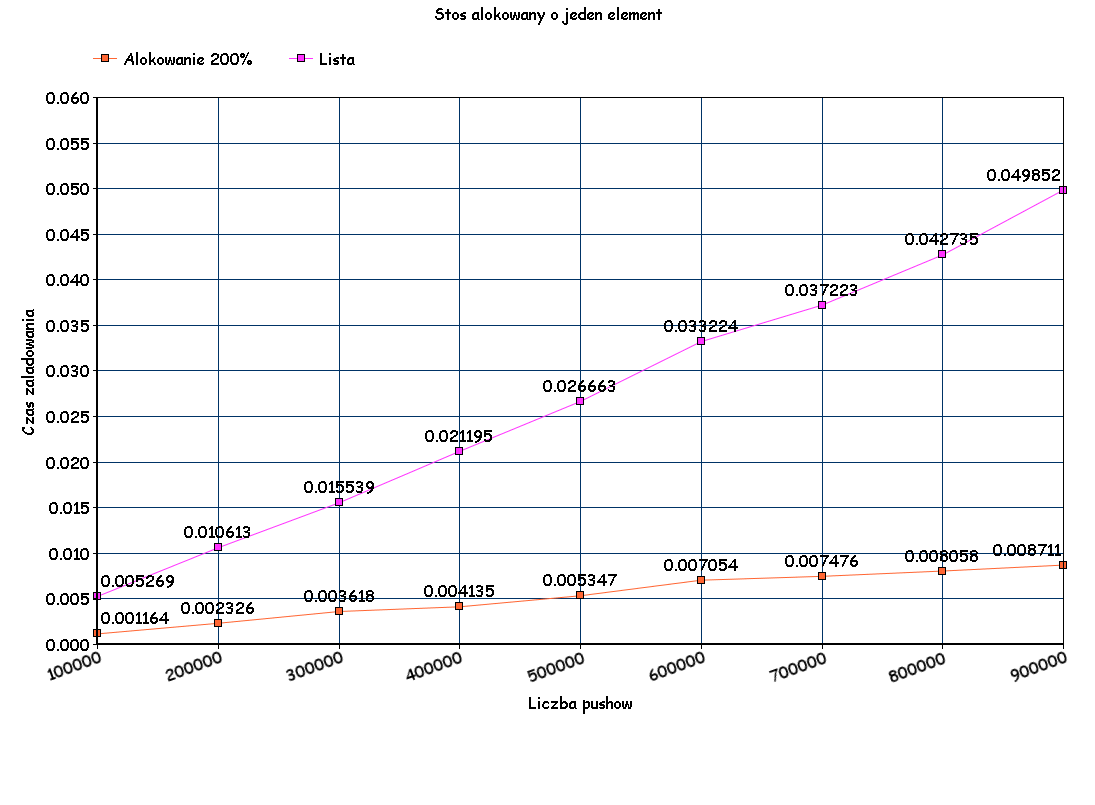
\includegraphics[width=6.5in]{3stos_dyn_o_200ilista.png}
Na podstawie wykresu można stwierdzić, że obie te implementacje mają przyrost liniowy
\section{Podsumowanie}
Pomimo dobrze opracowanej metody pomiarowej czasu, na wykresach widać zakłócenia spowodowane pracą programów w tle.


Najbardziej wydajnyą implementacją jest zoptymalizowany stos na tablicy(200\%), a następnie oprta na liście. Najdłuższy czas do przeprowadzaenia pushowania odnotowano przy niezoptymalizowanym stosie na tablicy, co jest spowodowane ciągłym kopiowaniem 
 elementów do nowej powiększonej tablicy.
\end{document}